
\chapter{Parametrization and Validation of Battery Models}

\section{Abstract}
This report presents results of parametrization and subsequent validation of a battery model using measured experimental data. Experimental recordings of slow charge and discharge cycle are used to estimate the open-circuit voltage $U_\text{OC}$ as a function of SOC. A pulse test is used to identify equivalent circuit model parameters $R_0$, $R_1$ and $C_1$. All estimates are verified using a testing data set with dynamic discharge profile.


\section{Open circuit voltage test}

During the identification experiment, the cell went through a full charge-discharge cycle using a small current of 120 mA. First, I wanted to include identification of hysteresis (both maximal magnitude as well as its dynamics represented by the decay rate $\gamma$), but I have given up on this task due to the limited amount of available data. Although it would be possible to estimate the maximal magnitude of hysteresis by simply subtracting the charging and discharging voltage curve and compensating the voltage drop on internal resistance, this piece of information would be worthless. The training data set lacks any sufficiently dynamic experiment where the hysteresis decay rate could be reliably identified, hence I would have to tune it using the validation data, which is against the point of validation.

Hence only the OCV curve as a function of SOC was obtained by averaging the voltage curve from charge and discharge half-cycle. All relevant curves can be seen in Fig. \ref{fig:6-ocv}.

\begin{figure}
    \centering
    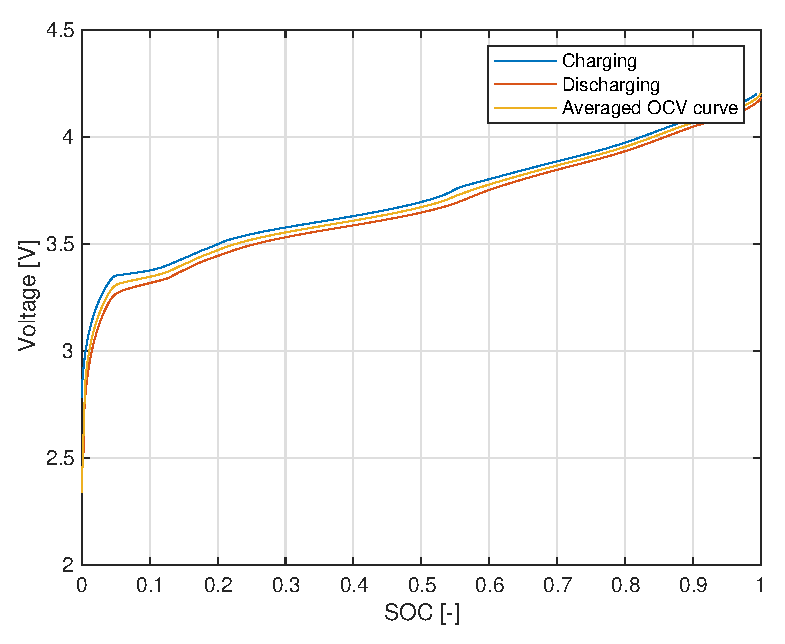
\includegraphics{figures/6/ocv.eps}
    \caption{Open circuit voltage as a function of SOC}
    \label{fig:6-ocv}
\end{figure}

\section{Identification of equivalent circuit model}

Estimated battery parameters are shown in Tab. \ref{tab:6-parameters}. The model achieved RMSE as low as 2.24 mV across the pulse experiment. This, combined with the degree of fit to training data shown in Fig. \ref{fig:6-pulse-compare} that is more than 86 \%, proves that the model indeed converged to reasonable parameters -- at least under the restriction of only 1 RC element. Adding more complexity to the model would improve its descriptive power and it would better match the system behavior.

The manual implementation of the discretized model was validated with results shown in Fig. \ref{fig:6-pulse-verification}. Since the results match the automatic comparison performed by Matlab, the model is implemented correctly.

\begin{figure}
    \centering
    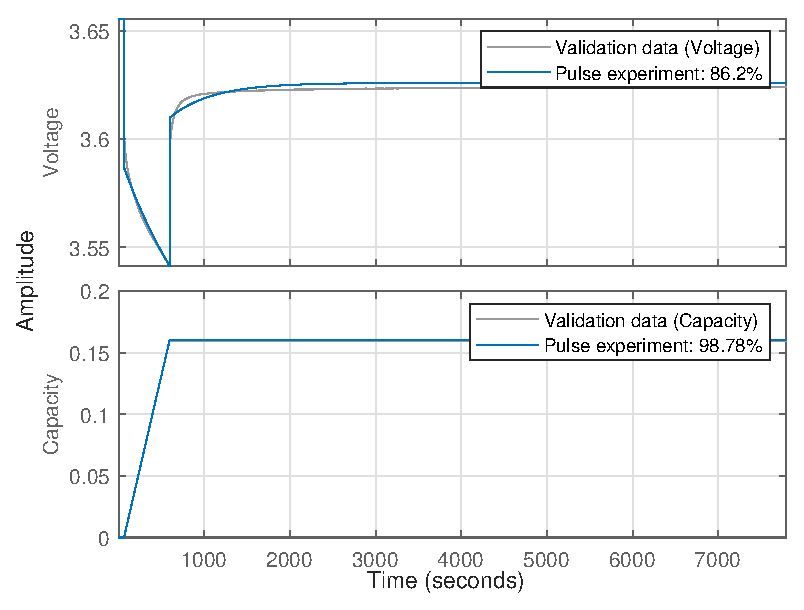
\includegraphics{figures/6/pulse-compare.eps}
    \caption{Assesment of model fit quality}
    \label{fig:6-pulse-compare}
\end{figure}

\begin{figure}
    \centering
    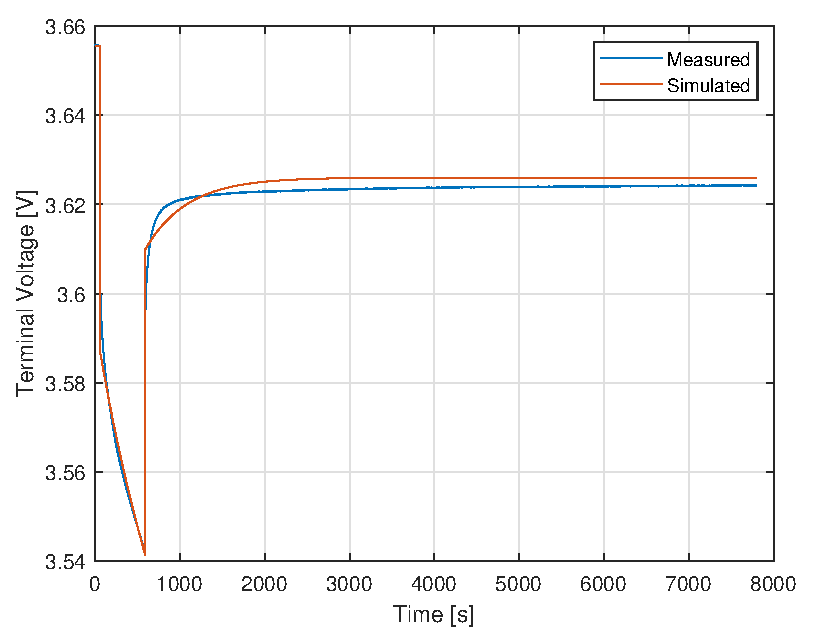
\includegraphics{figures/6/pulse-verification.eps}
    \caption{Manual comparison of model outputs and measurements}
    \label{fig:6-pulse-verification}
\end{figure}

\begin{table}[]
    \centering
    \begin{tabular}{c|c|c|c}
         Parameter & $R_0$ & $R_1$ & $C_1$ \\ \hline
         Value &  63.4e-3 $\Omega$ & 22.6e-3 $\Omega$ & 2.2e4 F 
    \end{tabular}
    \caption{Cell ECM parameters identified by the optimization procedure}
    \label{tab:6-parameters}
\end{table}

\section{Verification on dynamic discharge profile}

A provided DDP data set was used to verify model parameters identified in previous sections. The DDP consists of rapid discharge by constant 5.2 A, followed by discharge by 1.3 A and short charging by 2.5 A; everything in quick succession in 35 seconds. The model achieved RMSE of 47.3 mV across the whole experiment. Fig. \ref{fig:6-ddp-macro} shows that the model is indeed capable of capturing most of the cell dynamics, including gradual decrease of open circuit voltage. Some significant inaccuracy is still present however, as can be seen when zooming in on individual cycles of the DDP, as shown in Fig. \ref{fig:6-ddp-detail}. It is clear that the model failed to capture all system dynamics -- this is however expected since we have only used 1 RC element in the model. Adding a second one would improve the model fit to training data and decrease the RMSE on verification data. 

\begin{figure}
    \centering
    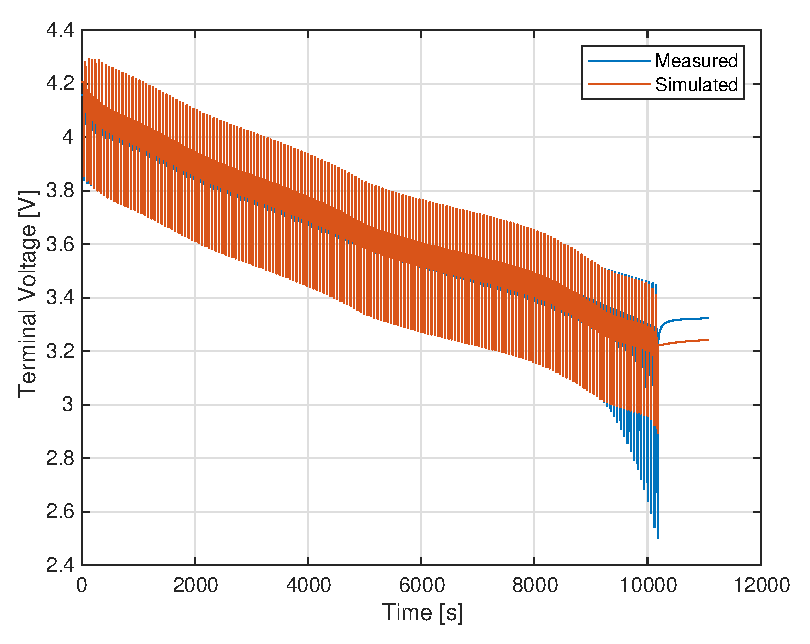
\includegraphics{figures/6/ddp-macro.eps}
    \caption{Comparison of measurements with simulated model outputs}
    \label{fig:6-ddp-macro}
\end{figure}

\begin{figure}
    \centering
    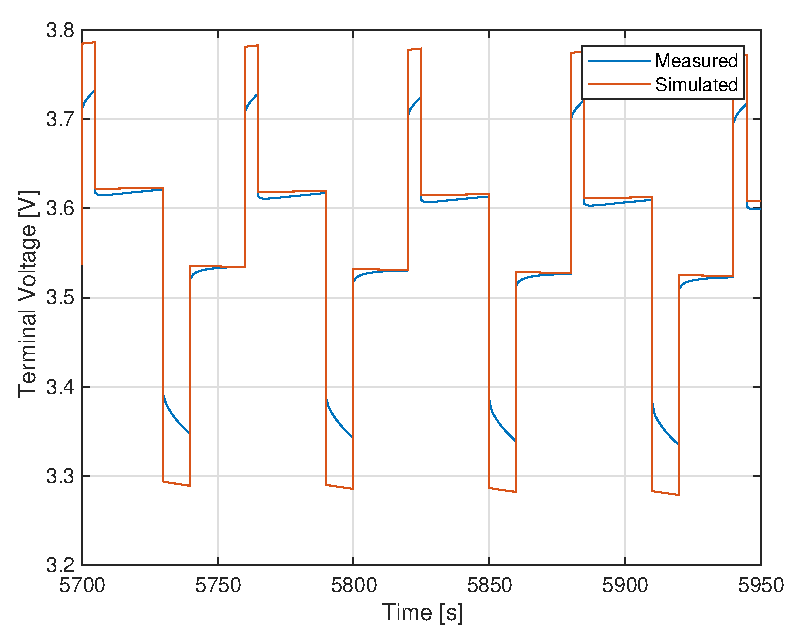
\includegraphics{figures/6/ddp-detail.eps}
    \caption{Verification of identified model on detail of several DDP cycles}
    \label{fig:6-ddp-detail}
\end{figure}

